\begin{exercice}[Quitte ou double]

À un jeu télévisé, la première bonne réponse rapporte 100\,€. Le gain double à chaque bonne réponse. Le candidat veut gagner plus de 100\,000\,€. À combien de questions doit-il répondre au minimum ? Détaille tes recherches. 
\end{exercice}

\begin{exercice}[Optimisation de la recherche]

\textbf{Femme :}  $L_F = T -100 -[T -150] / 2$ 

\textbf{Homme :} $L_H = T -100 -[T -150] / 4$ 

La formule de Lorentz permet d'associer la masse corporelle théorique $M$ (en kg) d'un adulte en fonction de sa taille $T$ (en cm), si celle-ci est comprise entre 140 et 220\,cm.

\begin{colenumerate}{1} 
\item Quelle est la masse corporelle théorique d'une femme mesurant 1,50\,m ? 1,60\,m ? 

Quelle est la taille idéale d'une femme dont la masse est 51\,kg ? 
\item Quelle est la masse corporelle théorique d'une homme mesurant 1,50\,m ? 1,90\,m ? 
 
 
Quelle est la taille idéale d'un homme dont la masse est 62 kg ? 
\end{colenumerate}
\end{exercice}

\begin{exercice}[Résolution graphique]

On recherche la(les) valeur(s) approchée(s) du(des) nombre(s) dont le carré vaut 0,5.

\begin{colenumerate}{1} 
\item Recopie et complète le tableau suivant :
 
%\renewcommand*\tabularxcolumn[1]{>{\centering\arraybackslash}m{#1}}
\begin{cltableau}{\linewidth}{8}
\hline
$x$ & $-1$ & $-0,9$ & $-0,8$ & ... & 0,8 & 0,9 & 1 \\ \hline
$x^2$ & & & & & & & \\ \hline
\end{cltableau}
 
\item Place dans un repère les points précédents en mettant $x$ en abscisse et $x^2$ en ordonnée (tu prendras 10\,cm pour une unité sur chaque axe).
\item Détermine graphiquement la(les) valeur(s) approchée(s) de $x$ pour laquelle $x^2 = 0,5$. Que remarques-tu ?
\end{colenumerate} 
\end{exercice}



\begin{exercice}[Énergie électrique]

\begin{cadre}
\textbf{Relations électriques}
\[ E = P\,t \]
\begin{itemize}
\item $E$ : Énergie électrique (en Wh)
\item $t$ : temps de fonctionnement (en h)
\item $P$ : Puissance consommée (en watts)
\[P = U\,I\]
\item $U$ : Tension (en volts)
\item $I$ : Intensité (en ampères)
\[U = R\,I\]
\item R : Résistance (en ohms)
\end{itemize}
\end{cadre}

Calcule la résistance d'un appareil fonctionnant sous une tension de 220\,volts pendant 45\,min et consommant une énergie de 1\,125\,Wh.
\end{exercice}




\begin{exercice}[Sécurité routière et distance d'arrêt]
(source : http://fr.wikipedia.org)

\includegraphics[width=\linewidth]{EqEA01}

\begin{enumerate} 
\item Temps de réaction et distance parcourue :

\begin{cadre}
\[ V = \dfrac{d_R}{t} \]
\begin{itemize} 
\item $V$ est la vitesse (en m/s)
\item $d_R$ est la distance de réaction (en m)
\item $t$ est le temps de réaction (en s)
\end{itemize}
\end{cadre}

Le temps de réaction d'un conducteur vigilant est d’environ 0,75\,s. Calcule la distance parcourue par un véhicule roulant à 100 km/h (27,8 m/s) pendant ce temps de réaction.

\item Distance de freinage :

\begin{cadre}
\[D_F = \dfrac{V^2}{2\,g\,A} \]
\begin{itemize}
\item $D_F$ : distance de freinage (en m)
\item $V$ : vitesse (en m/s)
\item $g$ = 9,81 (en N/kg)
\item $A$ : coefficient d'adhérence
\end{itemize}
\end{cadre}

Calcule la distance de freinage d'un véhicule roulant à 100\,km/h sur route sèche (coefficient d'adhérence $A = 0,6$). À quelle vitesse doit rouler ce même véhicule sur chaussée humide (coefficient d'adhérence $A = 0,4$) pour que sa distance de freinage reste inchangée.

\item Distance d'arrêt :

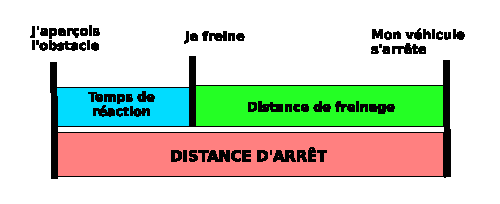
\includegraphics[width=\linewidth]{EqEA02}

Calcule la distance d'arrêt d'un véhicule roulant à 100\,km/h, dans la situation optimale (route sèche, plate et en bon état, freins performants, conducteur vigilant).

\item Autre méthode :

\[ D = \left(\dfrac{V}{10}\right)^2 \]

où $V$ est la vitesse exprimée en km/h.

Estime cette distance d'arrêt dans la situation optimale en utilisant la relation écrite ci-dessus.
\end{enumerate}
\end{exercice}
